
\documentclass{article}

\usepackage[version=3]{mhchem} % Package for chemical equation typesetting
\usepackage{siunitx} % Provides the \SI{}{} and \si{} command for typesetting SI units
\usepackage{graphicx} % Required for the inclusion of images
\usepackage{natbib} % Required to change bibliography style to APA
\usepackage{amsmath} % Required for some math elements 
\usepackage{caption}
\usepackage{subcaption}
\usepackage{listings}
\usepackage{color}
\usepackage{textcomp}
\definecolor{codegreen}{rgb}{0,0.6,0}
\definecolor{codegray}{rgb}{0.5,0.5,0.5}
\definecolor{codepurple}{rgb}{0.58,0,0.82}
\definecolor{backcolour}{rgb}{0.95,0.95,0.92}
 
\lstdefinestyle{mystyle}{
    backgroundcolor=\color{backcolour},   
    commentstyle=\color{codegreen},
    keywordstyle=\color{codepurple},
    numberstyle=\tiny\color{codegray},
    stringstyle=\color{codepurple},
    basicstyle=\footnotesize,
    breakatwhitespace=false,         
    breaklines=true,                 
    captionpos=b,                    
    keepspaces=true,                 
    numbers=left,                    
    numbersep=5pt,                  
    showspaces=false,                
    showstringspaces=false,
    showtabs=false,                  
    tabsize=2
}
\lstset{style=mystyle}

\setlength\parindent{0pt} % Removes all indentation from paragraphs

\renewcommand{\labelenumi}{\alph{enumi}.} % Make numbering in the enumerate environment by letter rather than number (e.g. section 6)

\newcommand\tab[1][0.5cm]{\hspace*{#1}}

%\usepackage{times} % Uncomment to use the Times New Roman font

\renewcommand{\thesubsection}{\thesection.\alph{subsection}}

%----------------------------------------------------------------------------------------
%	DOCUMENT INFORMATION
%----------------------------------------------------------------------------------------

\title{COMP 304: Assignment 3} % Title

\author{Berkay \textsc{Barlas}} % Author name

\date{\today} % Date for the report

\begin{document}

\maketitle % Insert the title, author and date

\begin{center}
\begin{tabular}{l r}
Date Performed: & April 15, 2019 \\ % Date the experiment was performed
Instructor: & Didem Unat % Instructor/supervisor
\end{tabular}
\end{center}

% If you wish to include an abstract, uncomment the lines below
% \begin{abstract}
% Abstract text
% \end{abstract}

%----------------------------------------------------------------------------------------
%	SECTION 1
%----------------------------------------------------------------------------------------


\section{Problem 1}
5 memory partitions of 100 KB, 500 KB, 200 KB, 300 KB, and 600KB (in order).
 How would you place the process of 212 KB, 417 KB, 112 KB, and 426 KB
\\
\\ \textbf{Which of these algorithms has the most efficient memory usage?}
\\ Best-fit algorithm is the most efficient one in terms of memory usage utilization.
\begin{description}
    \item[first-fit Algorithm] \hfill \\
    Allocate the first hole that is big enough.
    \\ 100KB $\,\to\,$ 
    \\ 500KB $\,\to\,$ 212KB
    \\ 200KB $\,\to\,$ 112KB
    \\ 300KB $\,\to\,$
    \\ 600KB $\,\to\,$ 417KB
    \\ Due to external fragmentation 426KB couldn't allocated.
     \item[best-fit Algorithm] \hfill \\
    Allocate the smallest hole that is big enough; must search entire list, unless ordered by size.
    \\This strategy produces the smallest leftover hole.
    \\ 100KB $\,\to\,$
    \\ 500KB $\,\to\,$ 417KB
    \\ 200KB $\,\to\,$ 112KB
    \\ 300KB $\,\to\,$ 212KB
    \\ 600KB $\,\to\,$ 426KB
    \item[worst-fit Algorithm] \hfill \\
    Allocate the largest hole; must also search entire list.
    \\ 100KB $\,\to\,$ 
    \\ 500KB $\,\to\,$ 417KB
    \\ 200KB $\,\to\,$ 
    \\ 300KB $\,\to\,$ 112KB
    \\ 600KB $\,\to\,$ 212KB
    \\ Due to external fragmentation 426KB couldn't allocated.
\end{description}

\section{Problem 2}
A system with 30-bit logical (virtual) address uses a two-level page table.
Logical addresses are split into an 8-bit top-level page table field, a 12-bit second-level page
table field, and an offset
%\begin{equation*}
 %   CPU utilisation  = 100 * \frac{{Total Time Spend on Processes}}{\mathrm{Total Time Spend on Execution}}
%\begin{center}\ce{}\end{center}
%\end{equation*}
\begin{description}
    \item[What is the size of a page in this system ?] \hfill \\ 
    \item[How many pages are there in the address space ?] \hfill \\ 
\end{description}

\newpage

\section{Problem 3 Paging}

\subsection{5 frames for process}
\begin{description}
    \item[LRU] \hfill \\ 
    Page fault number:\\
    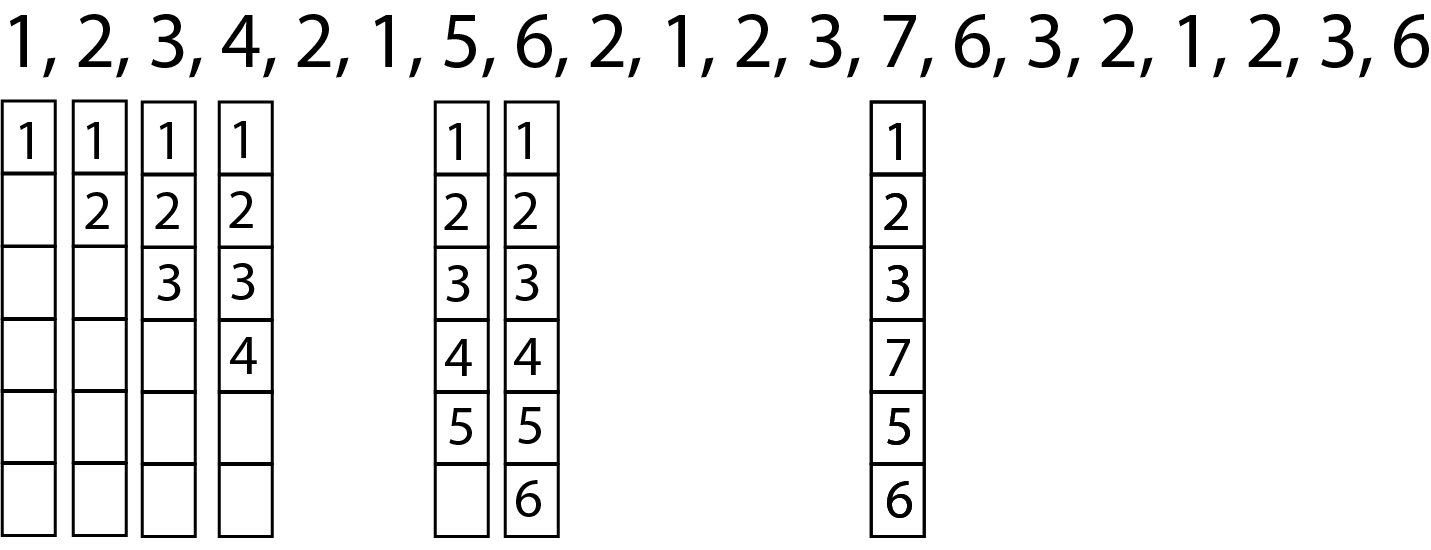
\includegraphics[width=1\linewidth]{./LRU6.png} 
    \item[FIFO] \hfill \\
    Page fault number:\\
    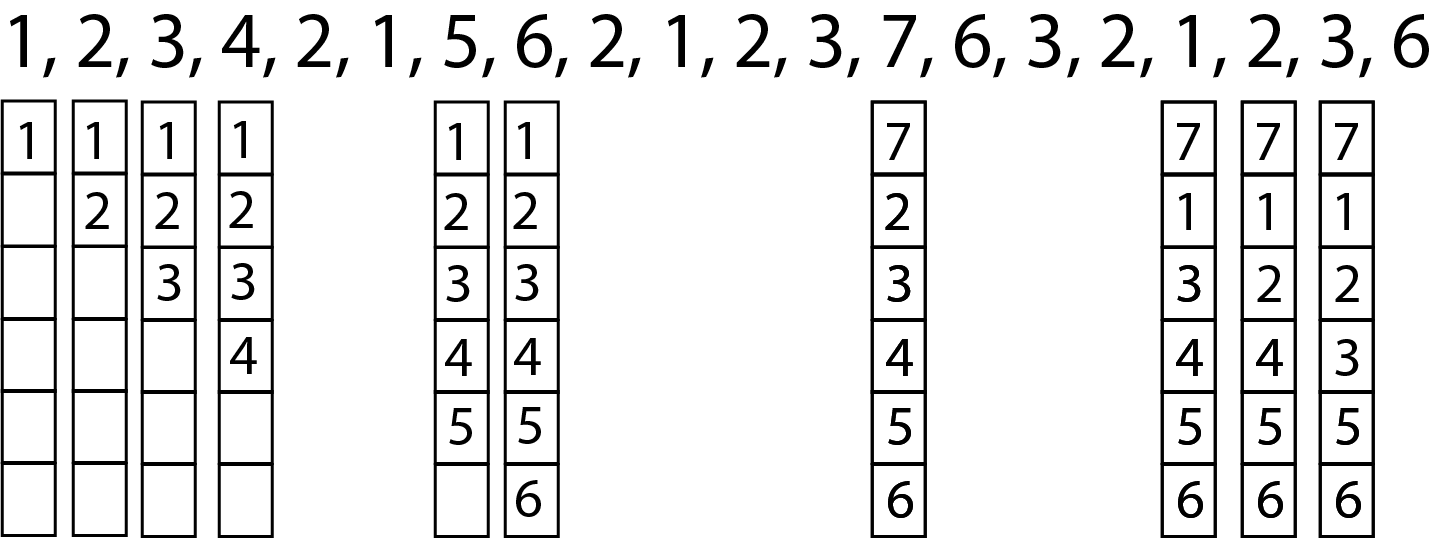
\includegraphics[width=1\linewidth]{./FIFO6.png} 
    \item[Optimal] \hfill \\
    Page fault number:\\
    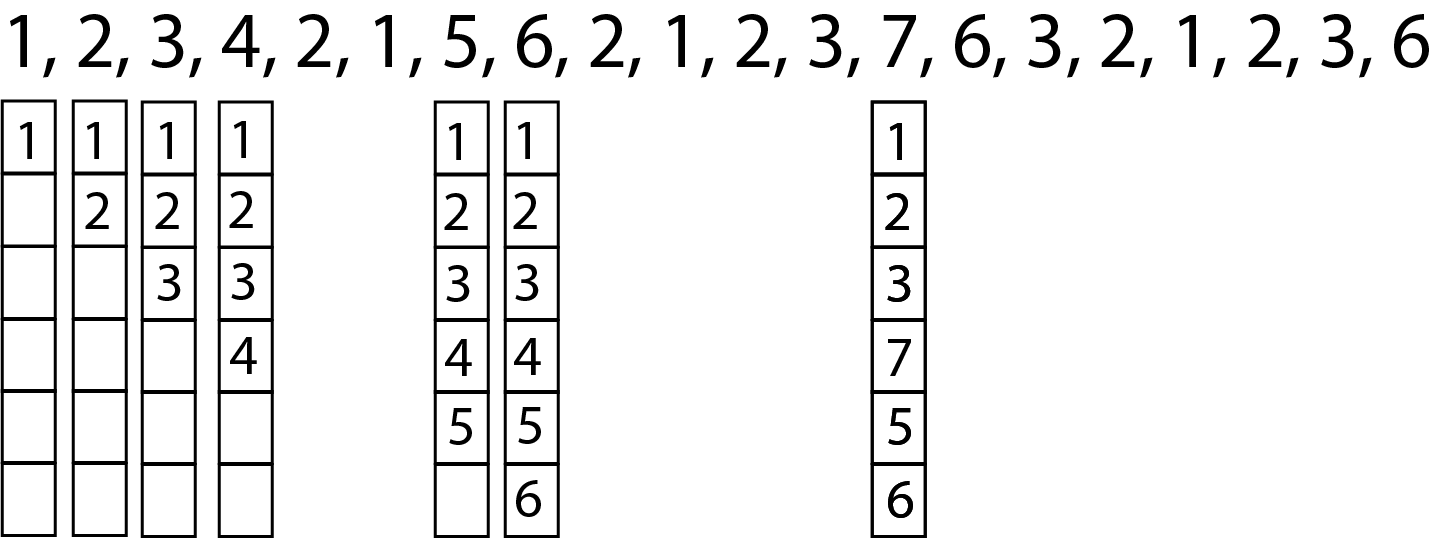
\includegraphics[width=1\linewidth]{./Optimal6.png} 
\end{description}
\subsection{6 frames for process}
\begin{description}
    \item[LRU] \hfill \\ 
    Page fault number:\\ 
    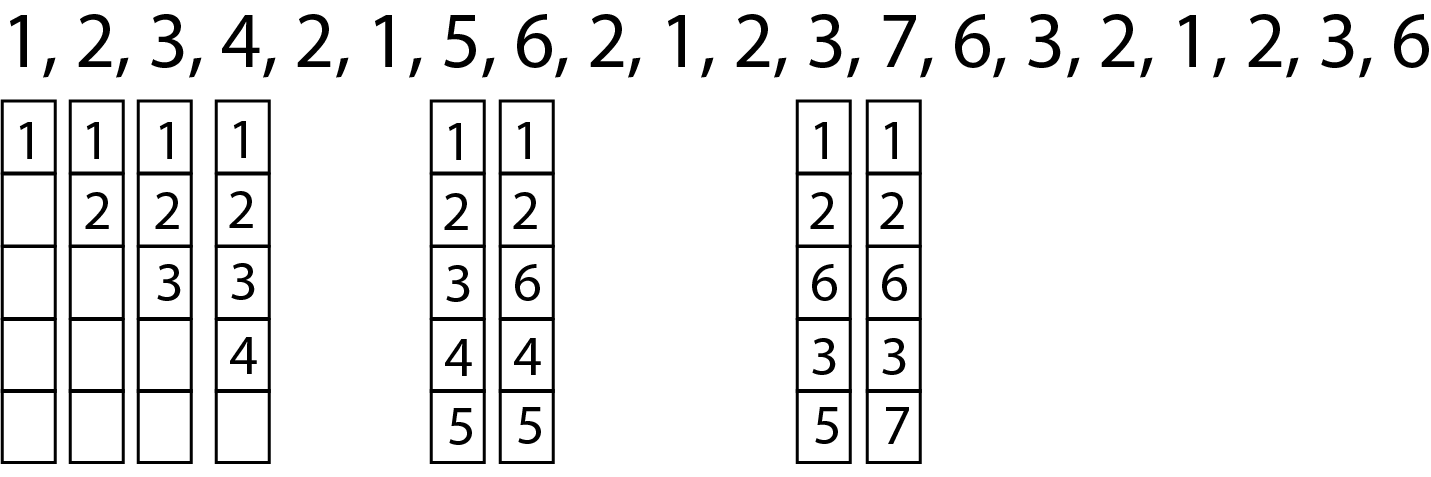
\includegraphics[width=1\linewidth]{./LRU5.png}
    \item[FIFO] \hfill \\
    Page fault number:\\ 
    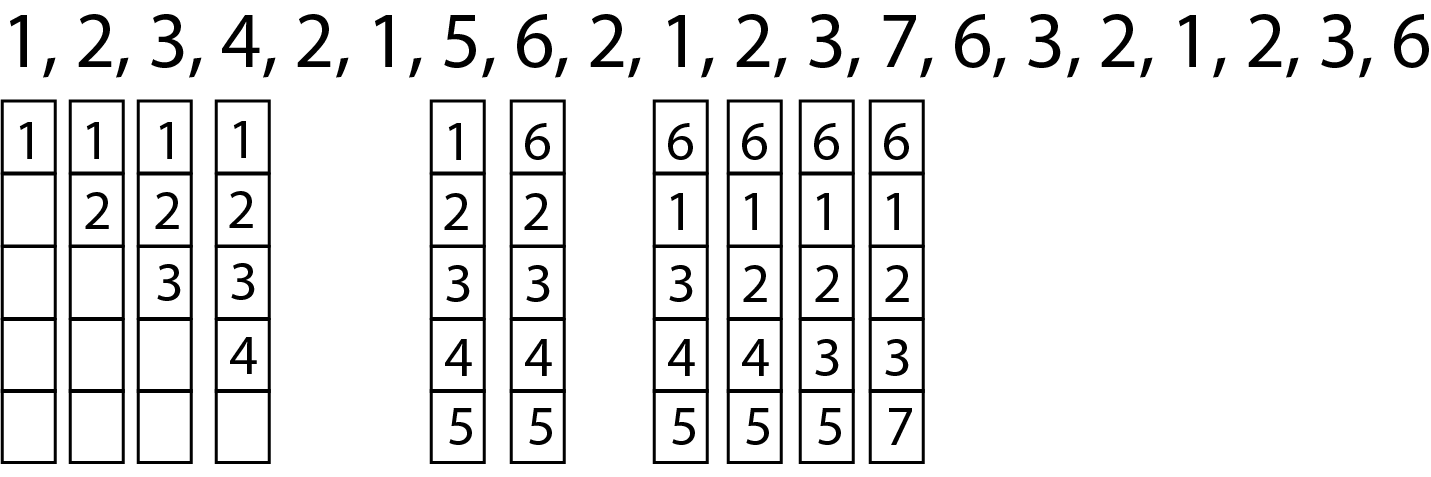
\includegraphics[width=1\linewidth]{./FIFO5.png}
    \item[Optimal] \hfill \\
    Page fault number:\\ 
    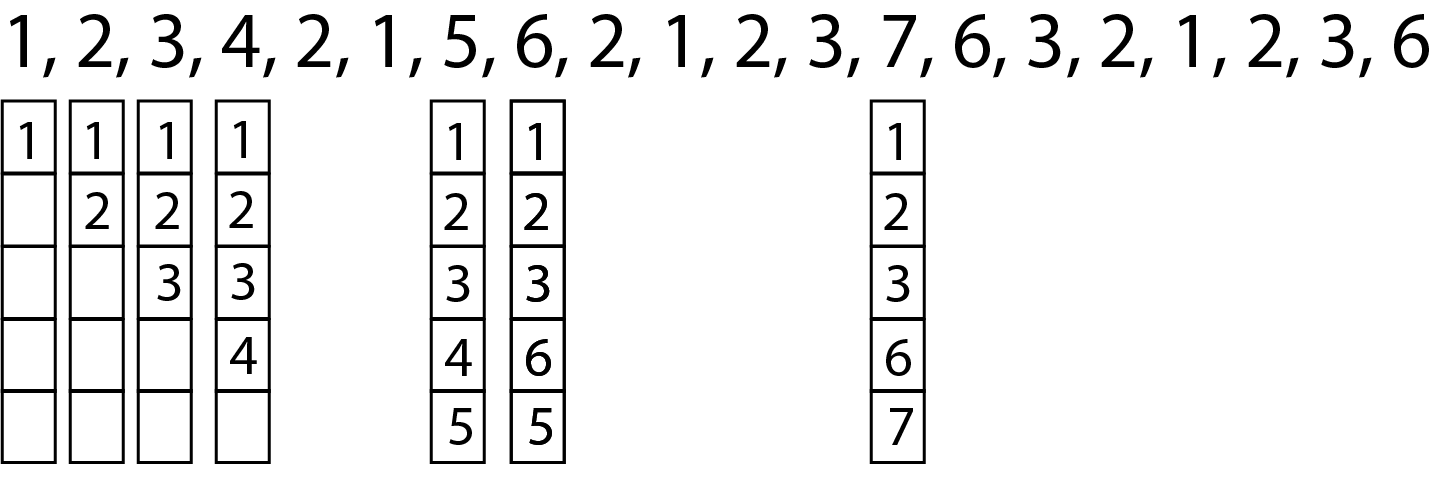
\includegraphics[width=1\linewidth]{./Optimal5.png}
\end{description}

\newpage
\section{Problem 4 Pure Demand Paging}
\subsection{Page fault rate when a process first starts execution}
\subsection{Page fault rate once the working set for a process is loaded into memory}
\subsection{Page fault rate when a process changes its locality and its new working set size is larger that the size of free memory}
\end{document}